% Aidan Hunt
% ME 498 K
% Spring 2023
% Homework 5

\documentclass{homework}
\usepackage[utf8]{inputenc}
\usepackage{amsmath}
\usepackage{amssymb}
\usepackage{braket}
\usepackage{bm}
\usepackage{caption}

% Packages for presenting code
\usepackage{listings}
\usepackage{pythonhighlight}


\lstdefinestyle{BashOutputStyle}{
  basicstyle=\footnotesize\ttfamily,
  numbers=none,
  frame=tblr,
  columns=fullflexible,
  backgroundcolor=\color{blue!10},
  linewidth=0.9\linewidth,
  xleftmargin=0.1\linewidth
}

% Packages for presenting output
\usepackage{hyperref}
\hypersetup{
    colorlinks=true,
    linkcolor=blue,
    filecolor=magenta,      
    urlcolor=blue,
    }

\raggedbottom

%use \question*{Title} to title a question

% make short commands for subproblem listing
\newcommand{\substart}{\begin{enumerate}[label={(\alph*)}]}
\newcommand{\subend}{\end{enumerate}}

%Instructor info
\newcommand{\hwname}{Aidan Hunt}
\newcommand{\hwemail}{ahunt94@uw.edu}

%Assignment type
\newcommand{\hwtype}{Homework}

%Class info
\newcommand{\hwclass}{ME 498 K}
\newcommand{\hwterm}{Spring 2023}

%Assignment specifics
\newcommand{\hwnum}{5}
\newcommand{\hwduedate}{May 5, 2023}

% \newcommand{\uu}	    {{\mathrm{\textbf{u}}}}

\begin{document}
\maketitle

In this homework, you will practice importing, manipulating, and analyzing Pandas DataFrames. Post questions about this assignment to the class discussion board for the fastest response. Submit your response as a single \texttt{.py} file (this is to encourage you to use an IDE with a variable viewer and debugger, like Spyder).

\subsubsection*{Background}

The Hydraulic Engineering Center's River Analysis System (HEC-RAS) is a tool for simulating river flows, and is useful for assessing how river channels, as well as structures in them like bridges and weirs, react to various flow profiles (like floods). We'll be looking at data from Spruce Creek and Bryon Creek in Pennsylvania. A simple discretized model of these creeks as implemented in HEC-RAS is shown below.

\begin{figure}[h]
    \centering
    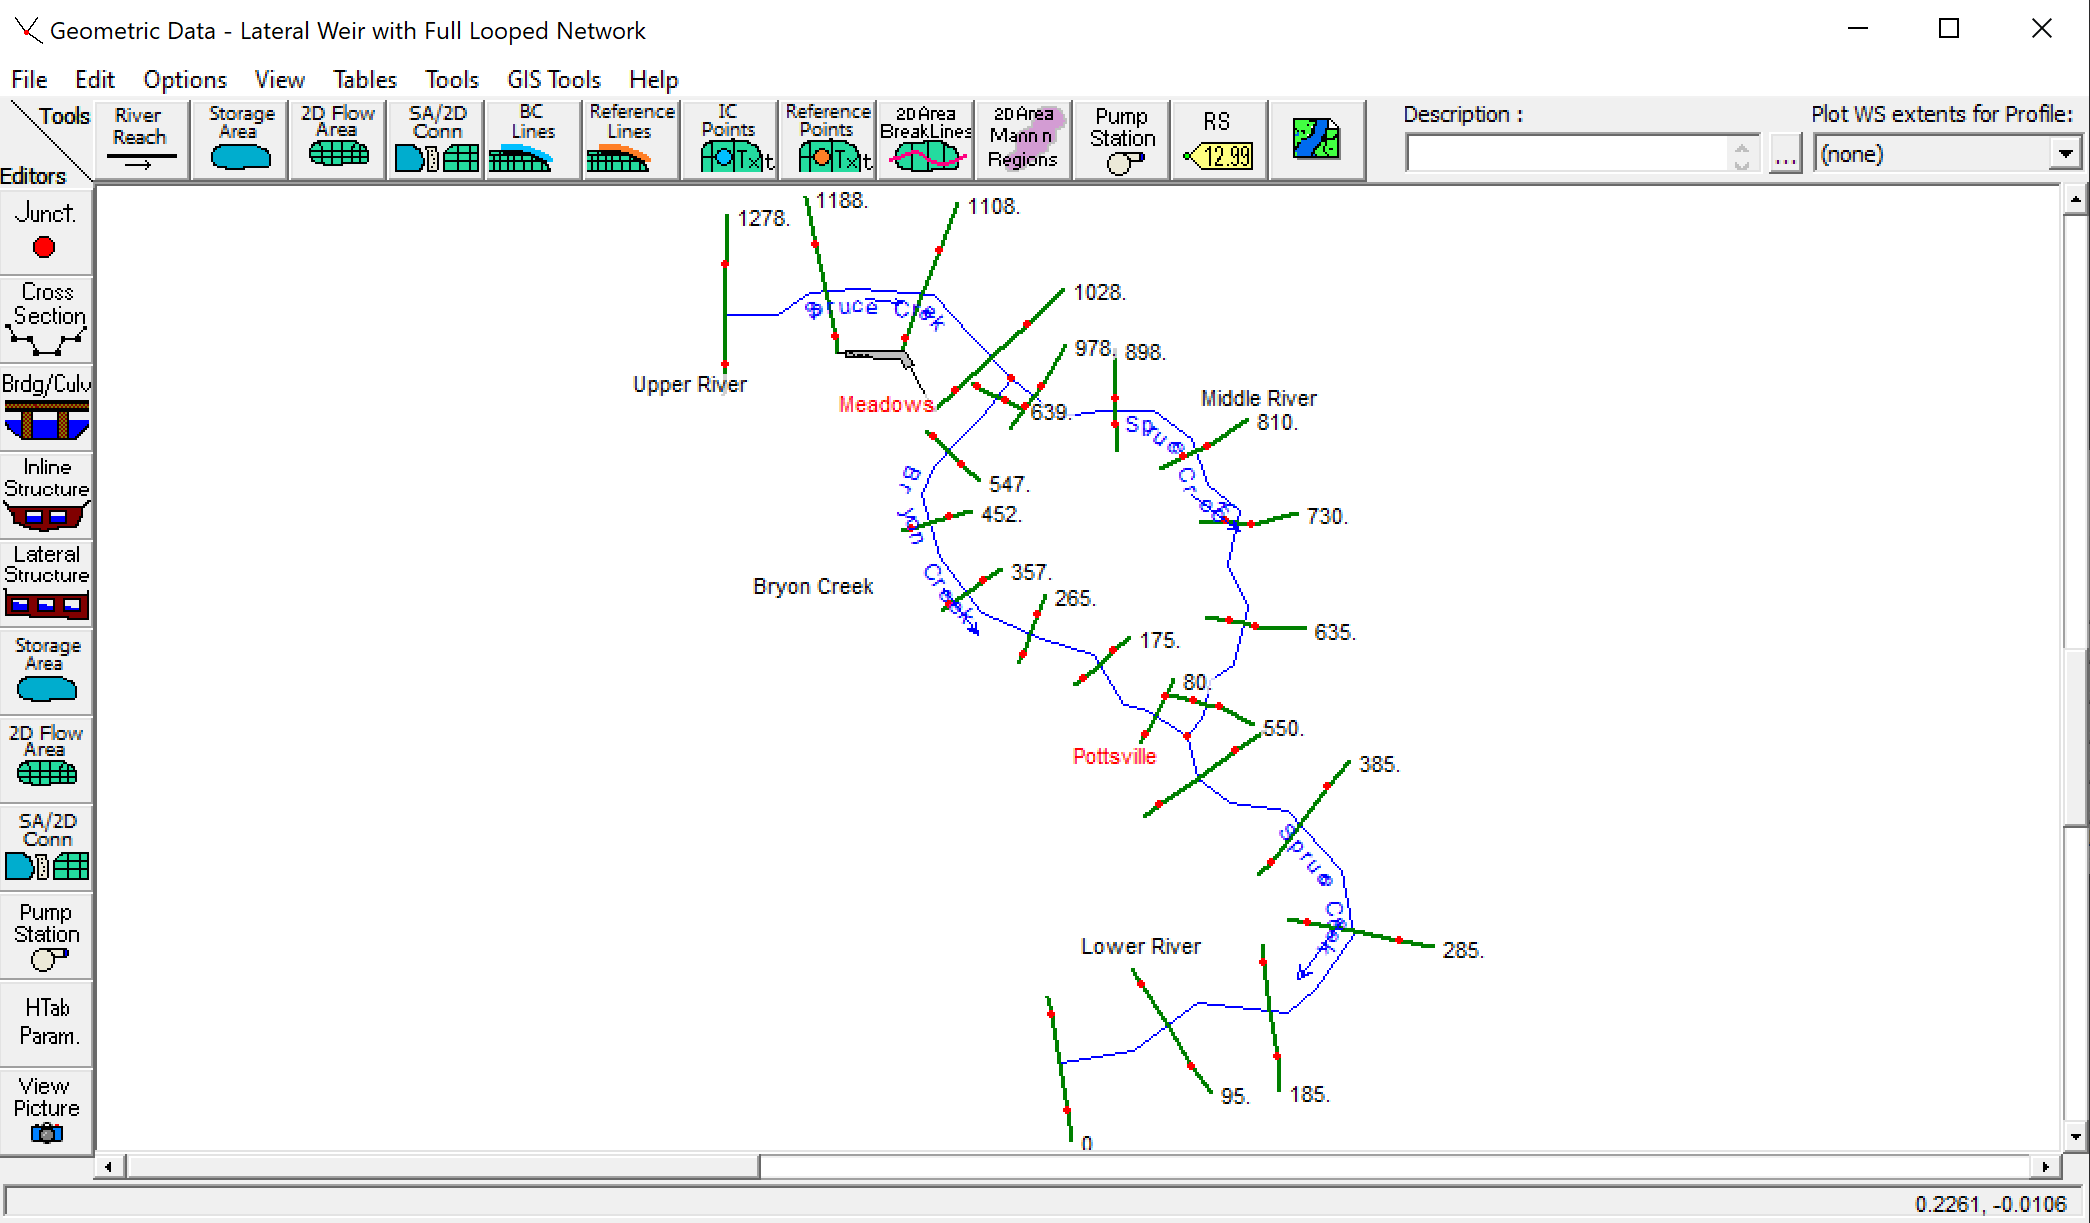
\includegraphics[width=0.8\textwidth]{hecras_geom.png}
\end{figure}

Below are the important points about this model for understanding the data you will work with:
\begin{itemize}
    \itemsep0em 
    \item There are several "river stations" labeled with numbers which indicate points along the river. The furthest upstream river station is "1278", and the furthest downstream station is "0".
    \item The blue lines represent the "rivers" (they are labeled "Spruce Creek" and "Bryon Creek").
    \item Spruce creek is split into three "reaches": "Upper River", "Middle River", and "Low River". Bryon Creek has only one reach, also named "Bryon Creek".
    \item Below the "Upper River" section of Spruce Creek, the creek splits into "Bryon Creek" and the "Middle River" section of Spruce Creek, before rejoining downstream as the "Lower River" of Spruce Creek.
\end{itemize}
Flow through these creeks is simulated in HEC-RAS for three flow profiles: "Low Water", "Standard Flow", and "Flood". HEC-RAS estimates several flow metrics at each river station, such as the total flow rate, water surface elevation, the velocity in the channel, and the Froude number. The resulting data is saved in \texttt{hecras\_flow\_split.txt}. This assignment has two main components. First, you will import the data into Python as a DataFrame using the Pandas package. Second, you will develop a single generalized plotting function to visualize various slices of this dataset.

% Insert image of channel layout
\subsubsection*{Importing the Data}

Your first task is to write a function that imports the data into Python using the Pandas package. 

\begin{python}
def importHECRAS(fileName):
    ''' docstring goes here '''
\end{python}

As in class, you should use the \href{https://pandas.pydata.org/docs/reference/api/pandas.read_csv.html}{\texttt{pd.read\_csv}} function to create a DataFrame from the HEC-RAS data. When using \texttt{pd.read\_csv}, you will need to specify values for several optional parameters:
\begin{itemize}
    \itemsep0em 
    \item You may assume that individual columns are separated by 2 or more space characters. Set the \texttt{delimiter} parameter to \texttt{'\textbackslash s\{2,\}'} and the \texttt{engine} parameter to \texttt{'python'}.
    \item You should ignore all content in the file before the first line of actual data, as well as any empty lines in the data (find the correct parameters to set in the \texttt{pd.read\_csv} documentation).
\end{itemize}

Additionally, your final DataFrame should have the following columns:
\begin{enumerate}
    \itemsep0em 
    \item "River" : Name of the river corresponding to each row of data.
    \item "Reach" : Name of the reach corresponding to each row of data.
    \item "Station" : River station number corresponding to each row of data.
    \item "Profile" : Name of the flow profile corresponding to each row of data.
    \item "Q" : Flow rate at each River/Reach/Station/Profile combination, in cfs
    \item "h" : Water surface (W. S.) elevation at each River/Reach/Station/Profile combination, in ft
    \item "V" : Velocity in the channel at each River/Reach/Station/Profile combination, in ft/s
    \item "Fr" : The Froude number at each River/Reach/Station/Profile combination (dimensionless)
\end{enumerate}
Note that this means we are only keeping a subset of the columns in the text file, and we are specifying the column names directly (there are a number of ways that you can accomplish these steps). You do not need to specify a new index for the DataFrame.

\subsubsection*{Visualizing the Data}

Your next task is to write a flexible plotting function for visualizing various flow metrics as a function of river station and flow profile. The river stations and flow profiles plotted will be chosen based on user inputs.

\begin{python}
def plotHECRAS(riverData, metric, riverName=None, reachName=None, profileName=None)
    ''' docstring goes here '''
\end{python}

Your function will take two required parameters: \texttt{riverData}, which is the full DataFrame as imported in the section above, and \texttt{metric}, which is a \texttt{str} that represents a particular flow metric we are interested in plotting. For example, a call to \texttt{plotHECRAS(riverData, 'Q')} would plot the flow rate \texttt{riverData['Q']} vs \texttt{riverData['Station']} for all rivers and profiles in \texttt{riverData} as in the plot shown.

\begin{figure}
    \centering
    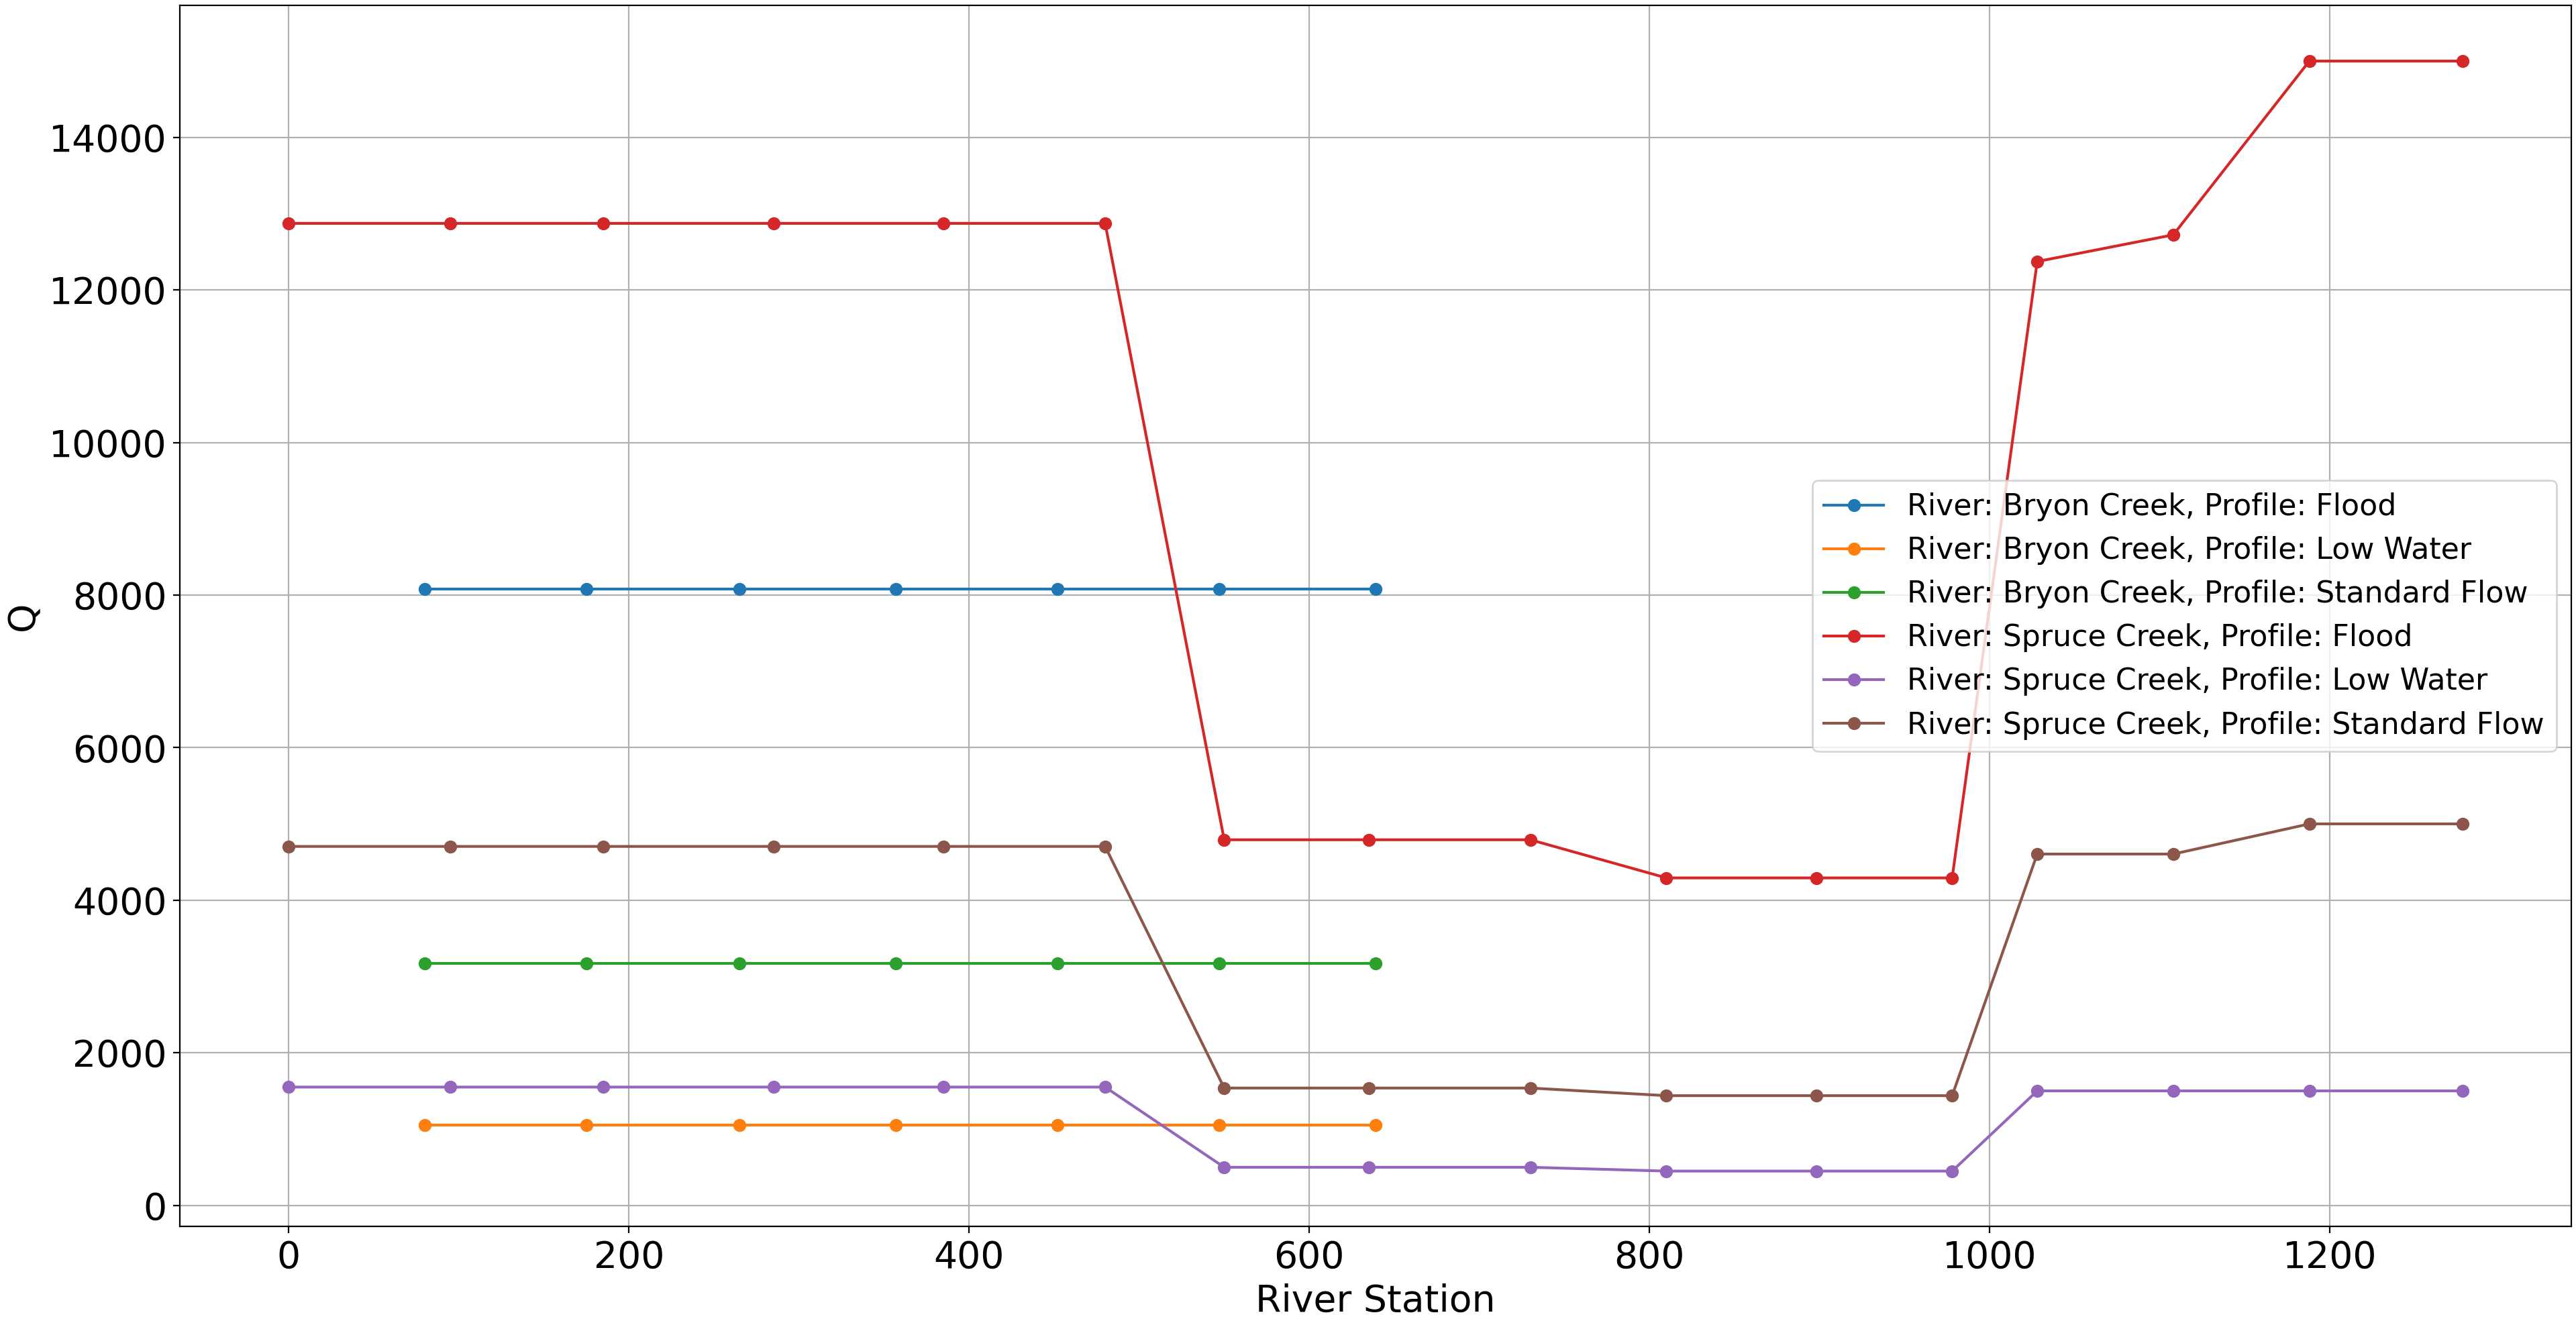
\includegraphics[width=0.8\textwidth]{defaultCase.png}
\end{figure}

However, your function will also take optional parameters \texttt{riverName}, \texttt{reachName}, and \texttt{profileName}. If the user specifies a particular river (case-sensitive), then only data corresponding to that river should be plotted. Similarly, if a reach is provided (case-sensitive), only data corresponding to river stations in that reach should be plotted. Similarly, if the user specifies a particular profile name (e.g., "Flood", case-sensitive), then only data corresponding to that profile should be plotted. To accomplish this, you will want to slice the rows of the input DataFrame according to the user inputs. \texttt{Examples of output plots with these optional inputs are posted on the Canvas page for this assignment}. 

As in past assignments, we want to handle cases in which the user provides invalid parameters. If the user inputs an invalid metric (i.e., a metric that is not \texttt{Q}, \texttt{h}, \texttt{V}, or \texttt{Fr}), your function should not produce any plots, and instead just print a message to the console saying that this column was not found in the input DataFrame. Similarly, if the user inputs invalid values for \texttt{riverName}, \texttt{reachName}, or \texttt{profileName}, or incompatible values for river and reach name (e.g., \texttt{riverName='Bryon Creek'} and \texttt{reachName='Upper River'}), your function should not produce any plots, and instead just print a message to the console indicating that slicing the data using these inputs results in an empty DataFrame. \textbf{You do not need to raise exceptions}; printing these messages is sufficient.

\lstinputlisting[style=BashOutputStyle]{badCol.txt}

\lstinputlisting[style=BashOutputStyle]{badSlice.txt}

Writing such a generalized function may seem daunting, but by outlining this in pseudocode, we can break this seemingly complex behavior down into several simpler cases. First, we only want to move forward with analysis if the user provided a valid metric, so we can check that right away. In the metric is indeed valid, we can then slice the DataFrame to include only the subset of rivers, reaches, and profiles based on the user's inputs (if provided). If there is something left to plot, we can do so. Otherwise, we can inform the user that the DataFrame is empty and end execution.

\begin{python}
def plotHECRAS(df, metric, riverName=None, reachName=None, profileName=None)
    ''' docstring goes here '''

    # If the provided metric is Q, h, V, or Fr
        # Slice the data frame based on the river name, if provided
        # Further slice the DataFrame based on the reach name, if provided
        # Further slice the DataFrame based on the given profile, if provided

        # If the final slice is not empty:
            # Plot metric vs river station for all rivers and profiles in the slice

        # Otherwise
            # Print message saying slice is empty

    # Otherwise
        # Print message saying metric is not in DataFrame
\end{python}

Additionally, note that slicing the DataFrame based on user inputs (but only if the user provided a value) is a similar task for the \texttt{riverName}, \texttt{reachName}, or \texttt{profileName} parameters...rather than copy/pasting similar value-checking code for all three of these parameters, we should write a flexible helper function that does this sort of "slice if user provided a value" task for us! You can use the following partially completed code; you only need to add a line of code that slices the DataFrame rows based on \texttt{colName} and \texttt{sliceVal}.

\begin{python}
def sliceIfValid(df, colName, sliceVal):
    '''
    Given an input DataFrame (df), slices the rows of df to include only
    those where the column given by the string colName is equal to the 
    value given by sliceVal. The sliced DataFrame is returned.

    If sliceVal is equal to None, or colName is not the name of a column
    in df, the original DataFrame is returned unsliced.
    '''

    if (sliceVal != None) and (colName in df.columns):
        # Slice the DataFrame somehow
    
    return df
\end{python}

\subsubsection*{Grading Criteria}

In terms of output, your code will be graded on whether it 1) correctly imports the HEC-RAS data as a DataFrame in the requested format, 2) correctly plots a requested metric (\texttt{Q}, \texttt{h}, \texttt{V}, or \texttt{Fr}) as a function of river station, and 3) correctly handles the optional inputs that may be provided by the user. The plots generated by your function should have \textbf{labeled $x$ and $y$ axes}, as well as a \textbf{legend denoting the river and profile of each line} (see example plot). Otherwise, there are no other formatting requirements for your plot.

In terms of style, your code should be well-structured and well-documented as always, and follow the Style Guide. You don't need to define more than the three functions described in this specification (you may define more if you would find it helpful), but \textbf{every} function must have a docstring that describes its parameters, returns, and other behavior. Remember, how your functions respond to both valid and invalid user input cases is important behavior that should be documented.

You should be able to accomplish the tasks in this assignment with the \texttt{pd.read\_csv} documentation and the slicing syntax we have used in class. If you need help with any aspect of this assignment, please post on the discussion board. Additionally, if you have any questions about general style requirements or the specific style requirements for this assignment, post them to the discussion board.

\end{document}

